% ACM DEBS Grand Challenge 2016
% Authors: author1, author2, author3, author4, author5, author6
%
% Style: SIG Proceedings Alternate VERSION 2.8

% You can indicate italicized words or phrases in your text with the command \texttt{{\char'134}textit}; emboldening with the command \texttt{{\char'134}textbf} and typewriter-style (for instance, for computer code) with \texttt{{\char'134}texttt}.

\documentclass{sig-alternate-05-2015}

\begin{document}

% COPYRIGHT
\setcopyright{acmcopyright}

% DOI
\doi{10.475/123_4}

% ISBN
\isbn{123-4567-24-567/08/06}

% CONFERENCE
\conferenceinfo{DEBS '16}{June 20--24, 2016, Irvine, CA, USA}

% PRICE
\acmPrice{\$15.00}

% AUTHOR METADATA
\conferenceinfo{DEBS}{'16 Irvine, California USA}
\CopyrightYear{2016} % Allows default copyright year (20XX) to be over-ridden - IF NEED BE.
%\crdata{0-12345-67-8/90/01}  % Allows default copyright data (0-89791-88-6/97/05) to be over-ridden - IF NEED BE.

% TITLE
\title{DEBS Grand Challenge: a processing engine for real-time analytics on social graph}

% AUTHORS
\numberofauthors{3}
\author{
% 1st. author
\alignauthor
Giacomo Marciani\\
\affaddr{University of Rome\\"Tor Vergata"}\\
\affaddr{Rome, Italy}\\
\email{giacomo.marciani\\@alumni.uniroma2.eu}
% 2nd. author
\alignauthor
Marco Piu\\
\affaddr{University of Rome\\"Tor Vergata"}\\
\affaddr{Rome, Italy}\\
\email{marco.piu\\@alumni.uniroma2.eu}
% 3rd. author
\alignauthor
Michele Porretta\\
\affaddr{University of Rome\\"Tor Vergata"}\\
\affaddr{Rome, Italy}\\
\email{michele.porretta\\@alumni.uniroma2.eu}
%\and
% 4th. author
}

\maketitle

% ABSTRACT
\begin{abstract}
Lorem ipsum dolor sit amet, consectetur adipiscing elit, sed do eiusmod tempor incididunt ut labore et dolore magna aliqua. Ut enim ad minim veniam, quis nostrud exercitation ullamco laboris nisi ut aliquip ex ea commodo consequat. Duis aute irure dolor in reprehenderit in voluptate velit esse cillum dolore eu fugiat nulla pariatur. Excepteur sint occaecat cupidatat non proident, sunt in culpa qui officia deserunt mollit anim id est laborum.
\end{abstract}

% CATEGORIES
% Should be generated by the tool at http://dl.acm.org/ccs.cfm
\begin{CCSXML}
<ccs2012>
	<concept>
		<concept_id>10010147.10010919.10010172</concept_id>
		<concept_desc>Computing methodologies~Distributed algorithms</concept_desc>
		<concept_significance>500</concept_significance>
	</concept>
</ccs2012>
\end{CCSXML}
\ccsdesc[500]{Computing methodologies~Distributed algorithms}

%  Use this command to print the description
\printccsdesc

% KEYWORDS
\keywords{ACM proceedings; Complex Event Processing; Event Stream Processing; Apache Storm; Amazon Web Services}

% INTRODUCTION
\section{Introduction}
Lorem ipsum dolor sit amet \cite{bowman:reasoning,braams:babel,clark:pct}, consectetur adipiscing elit, sed do eiusmod tempor incididunt ut labore et dolore magna aliqua. Ut enim ad minim veniam, quis nostrud exercitation ullamco laboris nisi ut aliquip ex ea commodo consequat. Duis aute irure dolor in reprehenderit in voluptate velit esse cillum dolore eu fugiat nulla pariatur. Excepteur sint occaecat cupidatat non proident, sunt in culpa qui officia deserunt mollit anim id est laborum.

\section{Solution}
Lorem ipsum dolor sit amet, consectetur adipiscing elit, sed do eiusmod tempor incididunt ut labore et dolore magna aliqua. Ut enim ad minim veniam, quis nostrud exercitation ullamco laboris nisi ut aliquip ex ea commodo consequat. Duis aute irure dolor in reprehenderit in voluptate velit esse cillum dolore eu fugiat nulla pariatur. Excepteur sint occaecat cupidatat non proident, sunt in culpa qui officia deserunt mollit anim id est laborum.

\begin{figure}
	\centering
	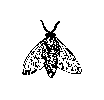
\includegraphics[height=1in, width=1in]{figures/fly}
	\caption{The topology.}
\end{figure}

\subsection{Query 1}
Lorem ipsum dolor sit amet, consectetur adipiscing elit, sed do eiusmod tempor incididunt ut labore et dolore magna aliqua. Ut enim ad minim veniam, quis nostrud exercitation ullamco laboris nisi ut aliquip ex ea commodo consequat. Duis aute irure dolor in reprehenderit in voluptate velit esse cillum dolore eu fugiat nulla pariatur. Excepteur sint occaecat cupidatat non proident, sunt in culpa qui officia deserunt mollit anim id est laborum.

\begin{figure}
	\centering
	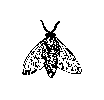
\includegraphics[height=1in, width=1in]{figures/fly}
	\caption{The topology for query 1.}
\end{figure}

\subsection{Query 2}
Lorem ipsum dolor sit amet, consectetur adipiscing elit, sed do eiusmod tempor incididunt ut labore et dolore magna aliqua. Ut enim ad minim veniam, quis nostrud exercitation ullamco laboris nisi ut aliquip ex ea commodo consequat. Duis aute irure dolor in reprehenderit in voluptate velit esse cillum dolore eu fugiat nulla pariatur. Excepteur sint occaecat cupidatat non proident, sunt in culpa qui officia deserunt mollit anim id est laborum.

\begin{figure}
	\centering
	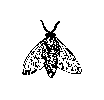
\includegraphics[height=1in, width=1in]{figures/fly}
	\caption{The topology for query 2.}
\end{figure}

\section{Evaluation}
Lorem ipsum dolor sit amet, consectetur adipiscing elit, sed do eiusmod tempor incididunt ut labore et dolore magna aliqua. Ut enim ad minim veniam, quis nostrud exercitation ullamco laboris nisi ut aliquip ex ea commodo consequat. Duis aute irure dolor in reprehenderit in voluptate velit esse cillum dolore eu fugiat nulla pariatur. Excepteur sint occaecat cupidatat non proident, sunt in culpa qui officia deserunt mollit anim id est laborum.

\begin{table}
	\centering
	\caption{Title goes here}
	\begin{tabular}{|c|c|l|}
		\hline
		Non-English or Math&Frequency&Comments\\ \hline
		\O & 1 in 1,000& For Swedish names\\ \hline
		$\pi$ & 1 in 5& Common in math\\ \hline
		\$ & 4 in 5 & Used in business\\ \hline
		$\Psi^2_1$ & 1 in 40,000& Unexplained usage\\
		\hline
	\end{tabular}
\end{table}

\subsection{Query 1}
Lorem ipsum dolor sit amet, consectetur adipiscing elit, sed do eiusmod tempor incididunt ut labore et dolore magna aliqua. Ut enim ad minim veniam, quis nostrud exercitation ullamco laboris nisi ut aliquip ex ea commodo consequat. Duis aute irure dolor in reprehenderit in voluptate velit esse cillum dolore eu fugiat nulla pariatur. Excepteur sint occaecat cupidatat non proident, sunt in culpa qui officia deserunt mollit anim id est laborum.

\subsection{Query 2}
Lorem ipsum dolor sit amet, consectetur adipiscing elit, sed do eiusmod tempor incididunt ut labore et dolore magna aliqua. Ut enim ad minim veniam, quis nostrud exercitation ullamco laboris nisi ut aliquip ex ea commodo consequat. Duis aute irure dolor in reprehenderit in voluptate velit esse cillum dolore eu fugiat nulla pariatur. Excepteur sint occaecat cupidatat non proident, sunt in culpa qui officia deserunt mollit anim id est laborum.

\section{Conclusions}
Lorem ipsum dolor sit amet, consectetur adipiscing elit, sed do eiusmod tempor incididunt ut labore et dolore magna aliqua. Ut enim ad minim veniam, quis nostrud exercitation ullamco laboris nisi ut aliquip ex ea commodo consequat. Duis aute irure dolor in reprehenderit in voluptate velit esse cillum dolore eu fugiat nulla pariatur. Excepteur sint occaecat cupidatat non proident, sunt in culpa qui officia deserunt mollit anim id est laborum.

\section{Acknowledgments}
Lorem ipsum dolor sit amet, consectetur adipiscing elit, sed do eiusmod tempor incididunt ut labore et dolore magna aliqua. Ut enim ad minim veniam, quis nostrud exercitation ullamco laboris nisi ut aliquip ex ea commodo consequat. Duis aute irure dolor in reprehenderit in voluptate velit esse cillum dolore eu fugiat nulla pariatur. Excepteur sint occaecat cupidatat non proident, sunt in culpa qui officia deserunt mollit anim id est laborum.

\section{Formatting examples}

\subsection{Math}
This is an inline equation

\begin{math}
	\lim_{n\rightarrow \infty}x=0
\end{math}

This is a display numbered equation

\begin{equation}
	\lim_{n\rightarrow \infty}x=0
\end{equation}

This is a display unnumbered equation:

\begin{displaymath}
	\sum_{i=0}^{\infty} x + 1
\end{displaymath}

\subsection{Theorem-like Constructs}
Other common constructs that may occur in your article are the forms for logical constructs like theorems, axioms, corollaries and proofs.  There are two forms, one produced by the command \texttt{{\char'134}newtheorem} and the other by the command \texttt{{\char'134}newdef}; perhaps the clearest and easiest way to distinguish them is to compare the two in the output of this sample document: This uses the \textbf{theorem} environment, created by the\linebreak\texttt{{\char'134}newtheorem} command:

\newtheorem{theorem}{Theorem}
\begin{theorem}
	Let $f$ be continuous on $[a,b]$.  If $G$ is an antiderivative for $f$ on $[a,b]$, then
	\begin{displaymath}
		\int^b_af(t)dt = G(b) - G(a).
	\end{displaymath}
\end{theorem}

The other uses the \textbf{definition} environment, created by the \texttt{{\char'134}newdef} command: \newdef{definition}{Definition}

\begin{definition}
	If $z$ is irrational, then by $e^z$ we mean the unique number which has logarithm $z$:
	\begin{displaymath}{\log e^z = z}\end{displaymath}
\end{definition}

Two lists of constructs that use one of these forms is given in the \textit{Author's  Guidelines}. There is one other similar construct environment, which is already set up for you; i.e. you must \textit{not} use a \texttt{{\char'134}newdef} command to create it: the \textbf{proof} environment.  Here is a example of its use:

\begin{proof}
	Suppose on the contrary there exists a real number $L$ such that
	\begin{displaymath}
		\lim_{x\rightarrow\infty} \frac{f(x)}{g(x)} = L.
	\end{displaymath}
	Then
	\begin{displaymath}
		l=\lim_{x\rightarrow c} f(x)
		= \lim_{x\rightarrow c}
		\left[ g{x} \cdot \frac{f(x)}{g(x)} \right ]
		= \lim_{x\rightarrow c} g(x) \cdot \lim_{x\rightarrow c}
		\frac{f(x)}{g(x)} = 0\cdot L = 0,
	\end{displaymath}
	which contradicts our assumption that $l\neq 0$.
\end{proof}

% REFERENCES
%Generated by bibtex from your ~.bib file.  Run latex,
%then bibtex, then latex twice (to resolve references)
%to create the ~.bbl file.  Insert that ~.bbl file into
%the .tex source file and comment out
%the command \texttt{{\char'134}thebibliography}.

\bibliographystyle{abbrv}
\bibliography{references}

\end{document}
